% Options for packages loaded elsewhere
\PassOptionsToPackage{unicode}{hyperref}
\PassOptionsToPackage{hyphens}{url}
%
\documentclass[
  ignorenonframetext,
]{beamer}
\usepackage{pgfpages}
\setbeamertemplate{caption}[numbered]
\setbeamertemplate{caption label separator}{: }
\setbeamercolor{caption name}{fg=normal text.fg}
\beamertemplatenavigationsymbolsempty
% Prevent slide breaks in the middle of a paragraph
\widowpenalties 1 10000
\raggedbottom
\setbeamertemplate{part page}{
  \centering
  \begin{beamercolorbox}[sep=16pt,center]{part title}
    \usebeamerfont{part title}\insertpart\par
  \end{beamercolorbox}
}
\setbeamertemplate{section page}{
  \centering
  \begin{beamercolorbox}[sep=12pt,center]{part title}
    \usebeamerfont{section title}\insertsection\par
  \end{beamercolorbox}
}
\setbeamertemplate{subsection page}{
  \centering
  \begin{beamercolorbox}[sep=8pt,center]{part title}
    \usebeamerfont{subsection title}\insertsubsection\par
  \end{beamercolorbox}
}
\AtBeginPart{
  \frame{\partpage}
}
\AtBeginSection{
  \ifbibliography
  \else
    \frame{\sectionpage}
  \fi
}
\AtBeginSubsection{
  \frame{\subsectionpage}
}

\usepackage{amsmath,amssymb}
\usepackage{iftex}
\ifPDFTeX
  \usepackage[T1]{fontenc}
  \usepackage[utf8]{inputenc}
  \usepackage{textcomp} % provide euro and other symbols
\else % if luatex or xetex
  \usepackage{unicode-math}
  \defaultfontfeatures{Scale=MatchLowercase}
  \defaultfontfeatures[\rmfamily]{Ligatures=TeX,Scale=1}
\fi
\usepackage{lmodern}
\ifPDFTeX\else  
    % xetex/luatex font selection
\fi
% Use upquote if available, for straight quotes in verbatim environments
\IfFileExists{upquote.sty}{\usepackage{upquote}}{}
\IfFileExists{microtype.sty}{% use microtype if available
  \usepackage[]{microtype}
  \UseMicrotypeSet[protrusion]{basicmath} % disable protrusion for tt fonts
}{}
\makeatletter
\@ifundefined{KOMAClassName}{% if non-KOMA class
  \IfFileExists{parskip.sty}{%
    \usepackage{parskip}
  }{% else
    \setlength{\parindent}{0pt}
    \setlength{\parskip}{6pt plus 2pt minus 1pt}}
}{% if KOMA class
  \KOMAoptions{parskip=half}}
\makeatother
\usepackage{xcolor}
\newif\ifbibliography
\setlength{\emergencystretch}{3em} % prevent overfull lines
\setcounter{secnumdepth}{-\maxdimen} % remove section numbering

\usepackage{color}
\usepackage{fancyvrb}
\newcommand{\VerbBar}{|}
\newcommand{\VERB}{\Verb[commandchars=\\\{\}]}
\DefineVerbatimEnvironment{Highlighting}{Verbatim}{commandchars=\\\{\}}
% Add ',fontsize=\small' for more characters per line
\usepackage{framed}
\definecolor{shadecolor}{RGB}{241,243,245}
\newenvironment{Shaded}{\begin{snugshade}}{\end{snugshade}}
\newcommand{\AlertTok}[1]{\textcolor[rgb]{0.68,0.00,0.00}{#1}}
\newcommand{\AnnotationTok}[1]{\textcolor[rgb]{0.37,0.37,0.37}{#1}}
\newcommand{\AttributeTok}[1]{\textcolor[rgb]{0.40,0.45,0.13}{#1}}
\newcommand{\BaseNTok}[1]{\textcolor[rgb]{0.68,0.00,0.00}{#1}}
\newcommand{\BuiltInTok}[1]{\textcolor[rgb]{0.00,0.23,0.31}{#1}}
\newcommand{\CharTok}[1]{\textcolor[rgb]{0.13,0.47,0.30}{#1}}
\newcommand{\CommentTok}[1]{\textcolor[rgb]{0.37,0.37,0.37}{#1}}
\newcommand{\CommentVarTok}[1]{\textcolor[rgb]{0.37,0.37,0.37}{\textit{#1}}}
\newcommand{\ConstantTok}[1]{\textcolor[rgb]{0.56,0.35,0.01}{#1}}
\newcommand{\ControlFlowTok}[1]{\textcolor[rgb]{0.00,0.23,0.31}{#1}}
\newcommand{\DataTypeTok}[1]{\textcolor[rgb]{0.68,0.00,0.00}{#1}}
\newcommand{\DecValTok}[1]{\textcolor[rgb]{0.68,0.00,0.00}{#1}}
\newcommand{\DocumentationTok}[1]{\textcolor[rgb]{0.37,0.37,0.37}{\textit{#1}}}
\newcommand{\ErrorTok}[1]{\textcolor[rgb]{0.68,0.00,0.00}{#1}}
\newcommand{\ExtensionTok}[1]{\textcolor[rgb]{0.00,0.23,0.31}{#1}}
\newcommand{\FloatTok}[1]{\textcolor[rgb]{0.68,0.00,0.00}{#1}}
\newcommand{\FunctionTok}[1]{\textcolor[rgb]{0.28,0.35,0.67}{#1}}
\newcommand{\ImportTok}[1]{\textcolor[rgb]{0.00,0.46,0.62}{#1}}
\newcommand{\InformationTok}[1]{\textcolor[rgb]{0.37,0.37,0.37}{#1}}
\newcommand{\KeywordTok}[1]{\textcolor[rgb]{0.00,0.23,0.31}{#1}}
\newcommand{\NormalTok}[1]{\textcolor[rgb]{0.00,0.23,0.31}{#1}}
\newcommand{\OperatorTok}[1]{\textcolor[rgb]{0.37,0.37,0.37}{#1}}
\newcommand{\OtherTok}[1]{\textcolor[rgb]{0.00,0.23,0.31}{#1}}
\newcommand{\PreprocessorTok}[1]{\textcolor[rgb]{0.68,0.00,0.00}{#1}}
\newcommand{\RegionMarkerTok}[1]{\textcolor[rgb]{0.00,0.23,0.31}{#1}}
\newcommand{\SpecialCharTok}[1]{\textcolor[rgb]{0.37,0.37,0.37}{#1}}
\newcommand{\SpecialStringTok}[1]{\textcolor[rgb]{0.13,0.47,0.30}{#1}}
\newcommand{\StringTok}[1]{\textcolor[rgb]{0.13,0.47,0.30}{#1}}
\newcommand{\VariableTok}[1]{\textcolor[rgb]{0.07,0.07,0.07}{#1}}
\newcommand{\VerbatimStringTok}[1]{\textcolor[rgb]{0.13,0.47,0.30}{#1}}
\newcommand{\WarningTok}[1]{\textcolor[rgb]{0.37,0.37,0.37}{\textit{#1}}}

\providecommand{\tightlist}{%
  \setlength{\itemsep}{0pt}\setlength{\parskip}{0pt}}\usepackage{longtable,booktabs,array}
\usepackage{calc} % for calculating minipage widths
\usepackage{caption}
% Make caption package work with longtable
\makeatletter
\def\fnum@table{\tablename~\thetable}
\makeatother
\usepackage{graphicx}
\makeatletter
\def\maxwidth{\ifdim\Gin@nat@width>\linewidth\linewidth\else\Gin@nat@width\fi}
\def\maxheight{\ifdim\Gin@nat@height>\textheight\textheight\else\Gin@nat@height\fi}
\makeatother
% Scale images if necessary, so that they will not overflow the page
% margins by default, and it is still possible to overwrite the defaults
% using explicit options in \includegraphics[width, height, ...]{}
\setkeys{Gin}{width=\maxwidth,height=\maxheight,keepaspectratio}
% Set default figure placement to htbp
\makeatletter
\def\fps@figure{htbp}
\makeatother

\makeatletter
\makeatother
\makeatletter
\makeatother
\makeatletter
\@ifpackageloaded{caption}{}{\usepackage{caption}}
\AtBeginDocument{%
\ifdefined\contentsname
  \renewcommand*\contentsname{Table of contents}
\else
  \newcommand\contentsname{Table of contents}
\fi
\ifdefined\listfigurename
  \renewcommand*\listfigurename{List of Figures}
\else
  \newcommand\listfigurename{List of Figures}
\fi
\ifdefined\listtablename
  \renewcommand*\listtablename{List of Tables}
\else
  \newcommand\listtablename{List of Tables}
\fi
\ifdefined\figurename
  \renewcommand*\figurename{Figure}
\else
  \newcommand\figurename{Figure}
\fi
\ifdefined\tablename
  \renewcommand*\tablename{Table}
\else
  \newcommand\tablename{Table}
\fi
}
\@ifpackageloaded{float}{}{\usepackage{float}}
\floatstyle{ruled}
\@ifundefined{c@chapter}{\newfloat{codelisting}{h}{lop}}{\newfloat{codelisting}{h}{lop}[chapter]}
\floatname{codelisting}{Listing}
\newcommand*\listoflistings{\listof{codelisting}{List of Listings}}
\makeatother
\makeatletter
\@ifpackageloaded{caption}{}{\usepackage{caption}}
\@ifpackageloaded{subcaption}{}{\usepackage{subcaption}}
\makeatother
\makeatletter
\@ifpackageloaded{tcolorbox}{}{\usepackage[skins,breakable]{tcolorbox}}
\makeatother
\makeatletter
\@ifundefined{shadecolor}{\definecolor{shadecolor}{rgb}{.97, .97, .97}}
\makeatother
\makeatletter
\makeatother
\makeatletter
\makeatother
\ifLuaTeX
  \usepackage{selnolig}  % disable illegal ligatures
\fi
\IfFileExists{bookmark.sty}{\usepackage{bookmark}}{\usepackage{hyperref}}
\IfFileExists{xurl.sty}{\usepackage{xurl}}{} % add URL line breaks if available
\urlstyle{same} % disable monospaced font for URLs
\hypersetup{
  pdftitle={Untitled},
  hidelinks,
  pdfcreator={LaTeX via pandoc}}

\title{Untitled}
\author{}
\date{}

\begin{document}
\frame{\titlepage}
\ifdefined\Shaded\renewenvironment{Shaded}{\begin{tcolorbox}[interior hidden, sharp corners, borderline west={3pt}{0pt}{shadecolor}, frame hidden, breakable, boxrule=0pt, enhanced]}{\end{tcolorbox}}\fi

\begin{frame}{はじめに}
\protect\hypertarget{ux306fux3058ux3081ux306b}{}
今回の講習は実行環境によってエラーが起きます\\
エラーが出た場合は遠慮なく講習を止めてください

\textbf{ソフトのインストールは公式で推奨された方法を可能な限り使ってください}

実行環境 macOS 12.6.6
\end{frame}

\begin{frame}{なぜインストールについて学ぶのか}
\protect\hypertarget{ux306aux305cux30a4ux30f3ux30b9ux30c8ux30fcux30ebux306bux3064ux3044ux3066ux5b66ux3076ux306eux304b}{}
開発を始める前には環境構築が重要です。

しかし環境構築にはさまざまな困難があり、開発を始めるにも一苦労します。

今回のインストールについて知識をつけることで、環境構築の手間を軽減できます。
\end{frame}

\begin{frame}{事前知識}
\protect\hypertarget{ux4e8bux524dux77e5ux8b58}{}
\end{frame}

\begin{frame}{人とパソコンは言語が違う}
\protect\hypertarget{ux4ebaux3068ux30d1ux30bdux30b3ux30f3ux306fux8a00ux8a9eux304cux9055ux3046}{}

\includegraphics[width=6.25in,height=\textheight]{image/human_hello.png}


\includegraphics[width=6.25in,height=\textheight]{image/pc_hello.png}

パソコンが理解できるデータを\textbf{バイナリーデータ}と言う
\end{frame}

\begin{frame}{プログラムは翻訳され実行される}
\protect\hypertarget{ux30d7ux30edux30b0ux30e9ux30e0ux306fux7ffbux8a33ux3055ux308cux5b9fux884cux3055ux308cux308b}{}

\includegraphics[width=8.33333in,height=\textheight]{image/intractive.png}

プログラムを翻訳する操作を\textbf{コンパイル}、\\
翻訳を行うソフトを\textbf{コンパイラー}と呼ぶ
\end{frame}

\begin{frame}[fragile]{プログラムも翻訳され実行される}
\protect\hypertarget{ux30d7ux30edux30b0ux30e9ux30e0ux3082ux7ffbux8a33ux3055ux308cux5b9fux884cux3055ux308cux308b}{}
C++のソースコード:

\begin{Shaded}
\begin{Highlighting}[]
\NormalTok{\#include \textless{}iostream\textgreater{}}

\NormalTok{int main() \{}
\NormalTok{    std::cout \textless{}\textless{} "hello!" \textless{}\textless{} std::endl;}
\NormalTok{    return 0;}
\NormalTok{\}}
\end{Highlighting}
\end{Shaded}

コードをバイナリーデータへ翻訳:

\begin{Shaded}
\begin{Highlighting}[]
\ExtensionTok{g++}\NormalTok{ hello.cpp }\AttributeTok{{-}o}\NormalTok{ hello}
\end{Highlighting}
\end{Shaded}

バイナリーデータの実行:

\begin{Shaded}
\begin{Highlighting}[]
\ExtensionTok{./hello}
\end{Highlighting}
\end{Shaded}

コンパイル言語:

\begin{Shaded}
\begin{Highlighting}[]
\ExtensionTok{./configure}
\FunctionTok{make}
\FunctionTok{make}\NormalTok{ install}
\end{Highlighting}
\end{Shaded}

インタプリンタ言語: ダウンロードしてパスを通す
\end{frame}

\begin{frame}{コンパイルの扱いは言語ごとに違う}
\protect\hypertarget{ux30b3ux30f3ux30d1ux30a4ux30ebux306eux6271ux3044ux306fux8a00ux8a9eux3054ux3068ux306bux9055ux3046}{}
\begin{itemize}[<+->]
\item
  コンパイル言語(Go、C++、Java)\\
  一度コンパイルしたファイルを使い回す
  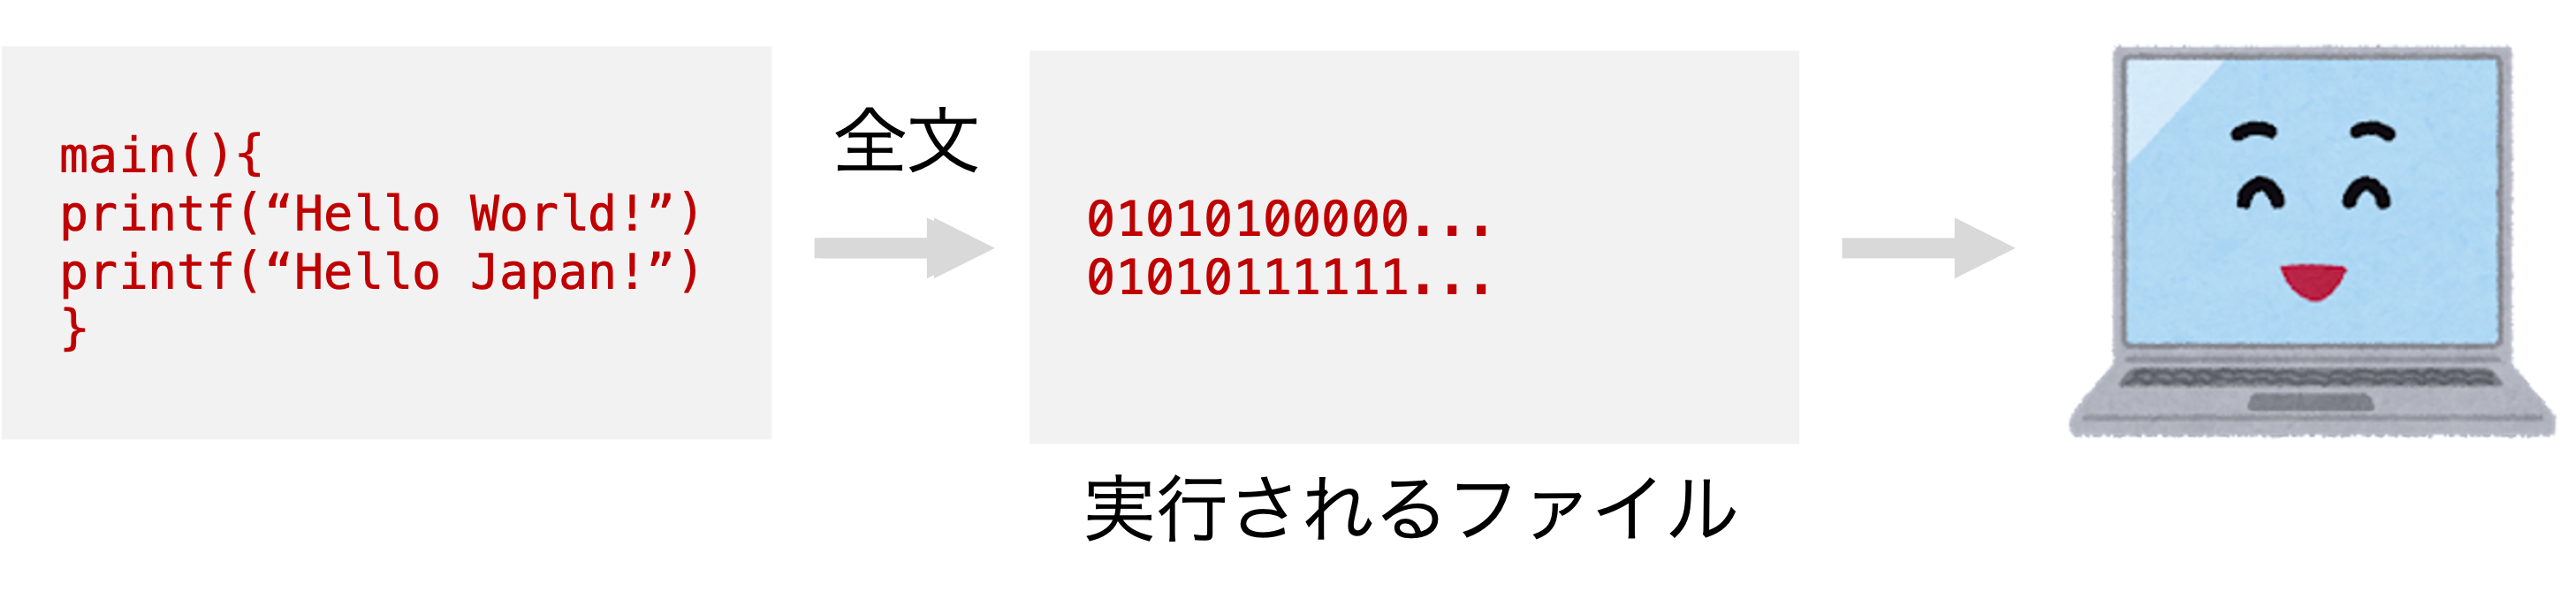
\includegraphics[width=9.375in,height=\textheight]{image/compile_language.png}
\item
  インタプリンタ言語(Python、R、Javascript)\\
  実行するたびにコンパイルする
  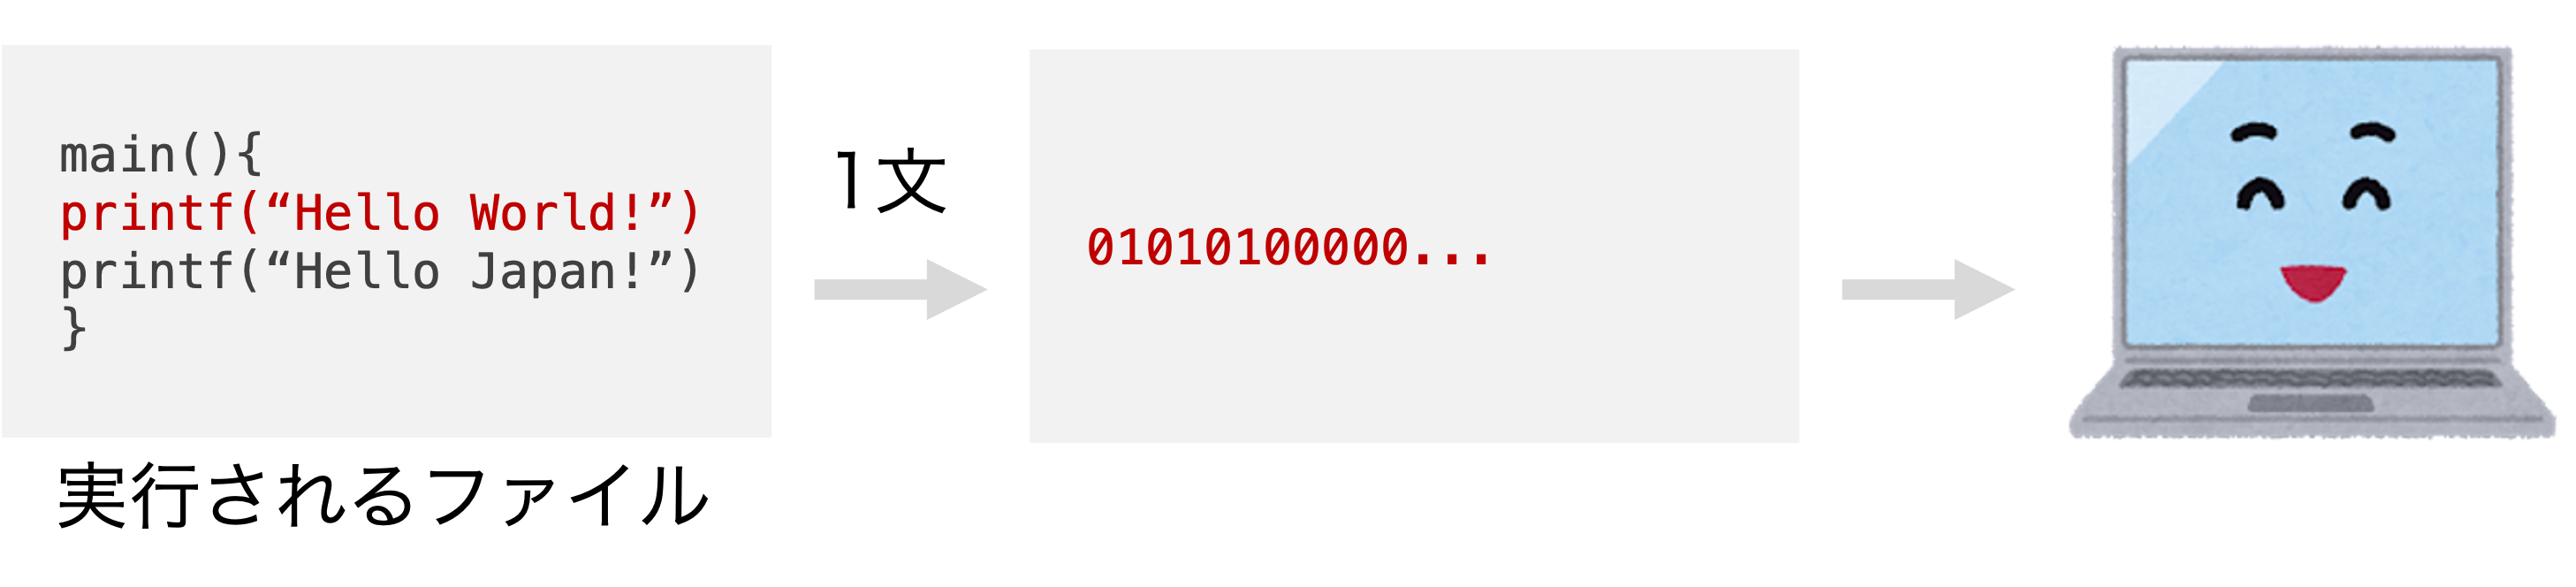
\includegraphics[width=9.375in,height=\textheight]{image/interprinter.png}
\end{itemize}
\end{frame}

\begin{frame}{インストールってなに?}
\protect\hypertarget{ux30a4ux30f3ux30b9ux30c8ux30fcux30ebux3063ux3066ux306aux306b}{}
ソフトウェアをパソコンへ導入し、使用可能な状態にする処理や作業のこと

ソフトウェアのインストールには大きくわけて2種の方法がある

\begin{itemize}[<+->]
\tightlist
\item
  ソースコードからソフトウェアを構築する\\
  (ソースからビルド)
\item
  パッケージマネージャーを使用する
\end{itemize}
\end{frame}

\begin{frame}{ソースコードからのインストール}
\protect\hypertarget{ux30bdux30fcux30b9ux30b3ux30fcux30c9ux304bux3089ux306eux30a4ux30f3ux30b9ux30c8ux30fcux30eb}{}
\begin{block}{コンパイル言語の場合:}
\protect\hypertarget{ux30b3ux30f3ux30d1ux30a4ux30ebux8a00ux8a9eux306eux5834ux5408}{}
\begin{enumerate}[<+->]
\tightlist
\item
  ソースコードのダウンロード
\item
  コンパイル用のファイルを作成(ない場合もある)
\item
  コンパイル実行
\item
  実行ファイルがある場所へパスを通す
\end{enumerate}
\end{block}

\begin{block}{インタプリンタ言語の場合:}
\protect\hypertarget{ux30a4ux30f3ux30bfux30d7ux30eaux30f3ux30bfux8a00ux8a9eux306eux5834ux5408}{}
\begin{enumerate}[<+->]
\tightlist
\item
  ソースコードのダウンロード
\item
  ダウンロードした場所へパスを通す
\end{enumerate}
\end{block}
\end{frame}

\begin{frame}[fragile]{コンパイル言語のインストール体験}
\protect\hypertarget{ux30b3ux30f3ux30d1ux30a4ux30ebux8a00ux8a9eux306eux30a4ux30f3ux30b9ux30c8ux30fcux30ebux4f53ux9a13}{}
\begin{enumerate}[<+->]
\tightlist
\item
  ソースコードのダウンロード
\end{enumerate}

\begin{Shaded}
\begin{Highlighting}[]
\FunctionTok{git}\NormalTok{ clone}
\end{Highlighting}
\end{Shaded}

\begin{enumerate}[<+->]
\setcounter{enumi}{1}
\tightlist
\item
  コンパイル用のファイル(Makefile)を作成:\\
\end{enumerate}

\begin{Shaded}
\begin{Highlighting}[]
\ExtensionTok{./configure}
\end{Highlighting}
\end{Shaded}

\begin{enumerate}[<+->]
\setcounter{enumi}{2}
\tightlist
\item
  コンパイル実行(実行ファイルを作成):\\
\end{enumerate}

\begin{Shaded}
\begin{Highlighting}[]
\FunctionTok{make}
\end{Highlighting}
\end{Shaded}
\end{frame}

\begin{frame}[fragile]{コンパイル言語のインストール体験}
\protect\hypertarget{ux30b3ux30f3ux30d1ux30a4ux30ebux8a00ux8a9eux306eux30a4ux30f3ux30b9ux30c8ux30fcux30ebux4f53ux9a13-1}{}
\begin{enumerate}[<+->]
\setcounter{enumi}{3}
\tightlist
\item
  パスを通す:\\
\end{enumerate}

\begin{Shaded}
\begin{Highlighting}[]
\BuiltInTok{pwd} \CommentTok{\#出力結果をコピー}
\FunctionTok{nano}\NormalTok{ \textasciitilde{}/zsh\_profile }\CommentTok{\#shellの種類に応じて\_の前を変更}

\CommentTok{\# zsh\_profile内の一番下の行に以下の内容を追記}
\VariableTok{PATH}\OperatorTok{=}\StringTok{"コピー内容をペースト:}\VariableTok{$PATH}\StringTok{"}
\end{Highlighting}
\end{Shaded}

プログラムの実行

\begin{Shaded}
\begin{Highlighting}[]
\ExtensionTok{prime}
\end{Highlighting}
\end{Shaded}

🔰 好きな整数を半角で入力し、素数判定を行う

🔰 ディレクトリを移動し\texttt{prime}を実行しよう
\end{frame}

\begin{frame}[fragile]{インタプリンタ言語のインストール体験}
\protect\hypertarget{ux30a4ux30f3ux30bfux30d7ux30eaux30f3ux30bfux8a00ux8a9eux306eux30a4ux30f3ux30b9ux30c8ux30fcux30ebux4f53ux9a13}{}
\begin{enumerate}[<+->]
\tightlist
\item
  pythonコードのダウンロード
\end{enumerate}

\begin{Shaded}
\begin{Highlighting}[]
\FunctionTok{git}\NormalTok{ clone}
\end{Highlighting}
\end{Shaded}

\begin{enumerate}[<+->]
\setcounter{enumi}{1}
\tightlist
\item
  パスを通す
\end{enumerate}

\begin{Shaded}
\begin{Highlighting}[]
\BuiltInTok{cd} 
\BuiltInTok{pwd} \CommentTok{\#出力結果をコピー}
\FunctionTok{nano}\NormalTok{ \textasciitilde{}/zsh\_profile }\CommentTok{\#shellの種類に応じて\_の前を変更}

\CommentTok{\# zsh\_profile内の一番下の行に以下の内容を追記}
\VariableTok{PATH}\OperatorTok{=}\StringTok{"コピー内容をペースト:}\VariableTok{$PATH}\StringTok{"}
\end{Highlighting}
\end{Shaded}

プログラムの実行

\begin{Shaded}
\begin{Highlighting}[]
\ExtensionTok{prime.py}
\end{Highlighting}
\end{Shaded}
\end{frame}

\begin{frame}[fragile]{余談:新しいコンパイルcmake}
\protect\hypertarget{ux4f59ux8ac7ux65b0ux3057ux3044ux30b3ux30f3ux30d1ux30a4ux30ebcmake}{}
これまでは\texttt{configure}で環境を読み取り、Makefileを作るのが一般的だった。\\
しかし最近は\texttt{cmake}を活用したMakefileの作成が主流

cmakeの特徴として以下のものが挙げられる * 高速 *
作成側とインストール側の両方でcmakeのインストールが必要
\end{frame}

\begin{frame}{パッケージマネージャーとは?}
\protect\hypertarget{ux30d1ux30c3ux30b1ux30fcux30b8ux30deux30cdux30fcux30b8ux30e3ux30fcux3068ux306f}{}
ソフトウェアのインストールやバージョン管理を行うソフトのこと

以下の利点がある * インストールをコマンド1つで行える *
アップデートの際、ソフトを消してインストールし直す必要がない *
インストールに必要なものを全て入れてくれる
\end{frame}

\begin{frame}{homebrewって何?}
\protect\hypertarget{homebrewux3063ux3066ux4f55}{}
\end{frame}

\begin{frame}{便利機能その1bottle}
\protect\hypertarget{ux4fbfux5229ux6a5fux80fdux305dux306euxff11bottle}{}
\end{frame}

\begin{frame}{便利機能その2tap}
\protect\hypertarget{ux4fbfux5229ux6a5fux80fdux305dux306euxff12tap}{}
\end{frame}

\begin{frame}{homebrewを使ったインストール}
\protect\hypertarget{homebrewux3092ux4f7fux3063ux305fux30a4ux30f3ux30b9ux30c8ux30fcux30eb}{}
\end{frame}

\begin{frame}{インストール時のエラー対応}
\protect\hypertarget{ux30a4ux30f3ux30b9ux30c8ux30fcux30ebux6642ux306eux30a8ux30e9ux30fcux5bfeux5fdc}{}
\begin{block}{gcc error}
\protect\hypertarget{gcc-error}{}
使用しているコンパイラーが古くコンパイルができない状態

対策法\\
* コンパイラーの更新を行う * バイナリーデータをダウンロードする
\end{block}
\end{frame}

\begin{frame}{コンパイラーのダウンロード}
\protect\hypertarget{ux30b3ux30f3ux30d1ux30a4ux30e9ux30fcux306eux30c0ux30a6ux30f3ux30edux30fcux30c9}{}
\end{frame}

\begin{frame}[fragile]{バイナリーデータのダウンロード}
\protect\hypertarget{ux30d0ux30a4ux30caux30eaux30fcux30c7ux30fcux30bfux306eux30c0ux30a6ux30f3ux30edux30fcux30c9}{}
一部のソフトウェアはコンパイル済みのデータを公開している\\
コンパイルできないならばコンパイル済みのものをダウンロードする

\begin{Shaded}
\begin{Highlighting}[]
\FunctionTok{wget}\NormalTok{ URL}
\end{Highlighting}
\end{Shaded}

パスを通す

\begin{Shaded}
\begin{Highlighting}[]

\end{Highlighting}
\end{Shaded}
\end{frame}

\begin{frame}{解決が難しい状況}
\protect\hypertarget{ux89e3ux6c7aux304cux96e3ux3057ux3044ux72b6ux6cc1}{}
\begin{itemize}[<+->]
\tightlist
\item
  管理者権限がない

  \begin{itemize}[<+->]
  \tightlist
  \item
    一部のパッケージマネージャーが使えずコンパイラーを更新できない
  \end{itemize}
\item
  必須のソフトの配布が終了している

  \begin{itemize}[<+->]
  \tightlist
  \item
    python2など古いソフトは一部機能がなくなったり書きかわったりしているため\\
    使えない場合がある
  \end{itemize}
\end{itemize}

\begin{block}{対応策}
\protect\hypertarget{ux5bfeux5fdcux7b56}{}
\begin{itemize}[<+->]
\tightlist
\item
  環境を変える

  \begin{itemize}[<+->]
  \tightlist
  \item
    DDBJからScorpionへ移動する
  \end{itemize}
\item
  別のソフトウェアを探す
\end{itemize}
\end{block}
\end{frame}



\end{document}
